\documentclass[11pt,letterpaper]{article}
\usepackage[lmargin=1in,rmargin=1in,tmargin=1in,bmargin=1in]{geometry}
\usepackage{../style/homework}
\usepackage{../style/commands}
\setbool{quotetype}{false} % True: Side; False: Under
\setbool{hideans}{false} % Student: True; Instructor: False

% -------------------
% Content
% -------------------
\begin{document}

\homework{7: Due 10/08}{I'm pretty but tough, like a diamond or beef jerky in a ball gown.}{Titus Andromedon, Unbreakable Kimmy Schmidt}


% Problem 1
\problem{10} Two functions $f(x)$ and $g(x)$ are plotted below. Are $f(x)$ and $g(x)$ functions? Explain. Do the functions $f(x)$ and $g(x)$ have an inverse? Explain.  
	\[
	\fbox{
	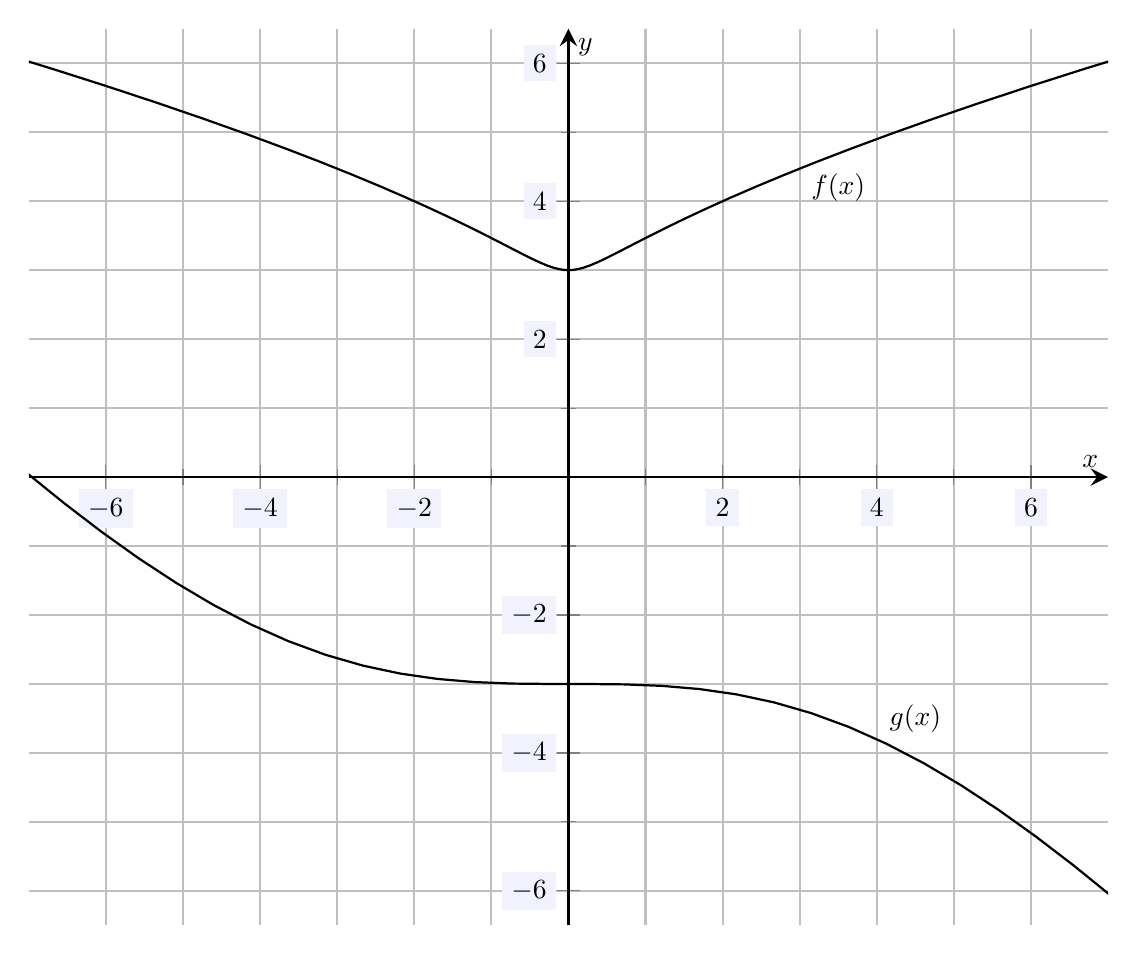
\begin{tikzpicture}[scale=2,every node/.style={scale=0.5}]
	\begin{axis}[
	grid=both,
	axis lines=middle,
	ticklabel style={fill=blue!5!white},
	xmin= -7, xmax=7,
	ymin= -6.5, ymax=6.5,
	xtick={-6,-4,-2,0,2,4,6},
	ytick={-6,-4,-2,0,2,4,6},
	minor tick = {-5,-3,...,5},
	xlabel=\(x\),ylabel=\(y\),
	]
	\node at (3.5,4.2) {$f(x)$};
	\addplot [domain= -3:3,samples=80] ({x^3 + x},{x^2 + 3}); 
	\node at (4.5,-3.5) {$g(x)$};
	\addplot [domain= -3:3,samples=100] ({8*x)},{-8*x^3/(x^2+1) - 3}); 
	\end{axis}
	\end{tikzpicture}
	}
	\] \pvspace{1.5cm}

{\itshape Because $f(x)$ and $g(x)$ pass the vertical line test, they are both functions. \pspace

Because $f(x)$ fails the horizontal line test and $g(x)$ passes the horizontal line test, $f(x)$ does not have an inverse whereas $g(x)$ does have an inverse.
}





\newpage





% Problem 2
\problem{10} Let $f(x)= 6x - 5$ and $g(x)= 2x^2 + 3x - 5$. 
	\begin{enumerate}[(a)]
	\item What is $g(2)$? 
	\item Assuming $g^{-1}$ exists, what is $g^{-1}(9)$?
	\item Assuming $f^{-1}$ exists, what is $f^{-1}(4)$?
	\end{enumerate} \pspace

\sol
{\itshape
\begin{enumerate}[(a)]
\item 
	\[
	g(2)= 2(2^2) + 3(2) - 5 = 2(4) + 6 - 5= 8 + 6 - 5= 14 - 5= 9
	\] \pspace


\item Because $g(2)= 9$, if $g^{-1}$ exists, then we must have $g^{-1}(9)= 2$ by the work from (a). \pspace


\item Suppose that $f^{-1}(4)= x$, then $f(x)= 4$. But then	
	\[
	\begin{aligned}
	6x - 5&= 4 \\[0.3cm]
	6x&= 9 \\[0.3cm]
	x&= \dfrac{9}{6} \\[0.3cm]
	x&= \dfrac{3}{2}
	\end{aligned}
	\]
\end{enumerate}
}





\newpage





% Problem 3
\problem{10} Do the points $(1, 3)$, $(3, 7)$, and $(5,1)$ lie along a line? Justify your answer. \pvspace{1.1cm}

\sol {\itshape Lines have constant slope. Therefore, if we compute the slope between these points, all the slopes computed should be the same. If this is so, then the points lie along a line. If all the slopes computed are not the same, then the points do not lie along a line. 
	\[
	\begin{aligned}
	m_1&= \dfrac{7 - 3}{3 - 1}= \dfrac{4}{2}= 2 \\[0.3cm]
	m_2&= \dfrac{1 - 7}{5 - 3}= \dfrac{-6}{2}= -3
	\end{aligned}
	\]
Because the slopes are not the same, the points do not lie along a line.}





\newpage





% Problem 4
\problem{10} Let $\ell(x)$ be the line through the points $(-2, 11)$ and $(3, -4)$.
	\begin{enumerate}[(a)]
	\item Find the slope of the line given by $\ell(x)$.
	\item Find the equation for $\ell(x)$.
	\item What is the $y$-intercept for $\ell(x)$?
	\item What is $\ell(-1)$?
	\end{enumerate} \pspace

\sol
{\itshape
\begin{enumerate}[(a)]
\item We have\dots
	\[
	m= \dfrac{-4 - 11}{3 - (-2)}= \dfrac{-4 - 11}{3 + 2}= \dfrac{-15}{5}= -3
	\] \pspace


\item The line is not vertical so that we know the line `looks like' $y= mx + b$. From (a), we know that $m= -3$. But then using the fact that $(-2, 11)$ is on the line, we have
	\[
	\begin{aligned}
	y= -3x + b \\
	11&= -3(-2) + b \\
	11&= 6 + b \\
	b&= 5
	\end{aligned}
	\]
Therefore, the equation of the line is $y= -3x + 5$, i.e. $y= 5 - 3x$. Using the `$\ell$' notation, we have $\ell(x)= -3x + 5$ or $\ell(x)= 5 - 3x$. \pspace


\item The $y$-intercept occurs when the curve passes through the $y$-axis, i.e. when $x= 0$. But then $\ell(0)= -3(0) + 5= 0 + 5= 5$. Therefore, the $y$-intercept is $(0, 5)$. \pspace

\item We have\dots
	\[
	\ell(-1)= -3(-1) + 5= 3 + 5= 8 
	\]
\end{enumerate}
}




\newpage





% Problem 5
\problem{10} Let $\ell(x)$ be the line through the point $(1, 3)$ with slope $\frac{1}{2}$.
	\begin{enumerate}[(a)]
	\item Find the equation for $\ell(x)$. 
	\item What is $\ell(4)$?
	\item Find the $x$-intercept for $\ell(x)$. 
	\end{enumerate} \pspace

\sol
{\itshape
\begin{enumerate}[(a)]
\item We know that the line is not vertical so that the line `looks like' $y= mx + b$. We know the slope is $m= \frac{1}{2}$. Then we know $y= \frac{1}{2} x + b$. But the line contains the point $(1, 3)$, so that
	\[
	\begin{aligned}
	y&= \frac{1}{2}x + b \\
	3&= \frac{1}{2} \cdot 1 + b \\
	3&= \frac{1}{2} + b \\
	b&= 3 - \frac{1}{2} \\
	b&= \frac{6}{2} - \frac{1}{2} \\
	b&= \frac{5}{2} 
	\end{aligned}
	\]
Therefore, $y= \frac{1}{2}x + \frac{5}{2}$ or equivalently $y= \frac{x + 5}{2}$. Using the `$\ell$' notation, we have $\ell(x)= \frac{1}{2}x + \frac{5}{2}$ or equivalently $\ell(x)= \frac{x + 5}{2}$. \pspace


\item We have\dots
	\[
	\ell(4)= \dfrac{1}{2} \cdot 4 + \dfrac{5}{2}= 2 + \dfrac{5}{2}= \dfrac{4}{2} + \dfrac{5}{2}= \dfrac{9}{2}
	\] \pspace


\item The $x$-intercept is when the curve passes through the $x$-axis, i.e. when $y= 0$. But then we have
	\[
	\begin{aligned}
	\dfrac{1}{2}x + \dfrac{5}{2}&= 0 \\
	\dfrac{1}{2}x&= -\dfrac{5}{2} \\
	x&= -5
	\end{aligned}
	\]
Therefore, the $x$-intercept is $(-5, 0)$. 
\end{enumerate}
}





\newpage





% Problem 6 
\problem{10} Determine if the following pairs of lines are parallel, perpendicular, or neither.
	\begin{enumerate}[(a)]
	\item $y= 5x$, \enskip $\frac{1}{5}x + y= 8$
	\item $x - 3y= 12$, \enskip $y= x + 7$
	\item $y= 3x - 1$, \enskip $6x - 2y= 4$
	\end{enumerate} \pspace

\sol
{\itshape
\begin{enumerate}[(a)]
\item The slope of $y= 5x$ is $m= 5$. For the second line, we solve for $y$: $y= 8 - \frac{1}{5} x$. Then the slope of this line is $m= -\frac{1}{5}$. Because $-\frac{1}{5}$ is the negative reciprocal of 5, the lines are perpendicular. \pspace


\item Solving for $y$ in the first line, we have $y= \frac{1}{3}x - 4$. Then this line has slope $m= \frac{1}{3}$. The slope of the line $y= x + 7$ is $m= 1$. Now $\frac{1}{3} \neq 1$ so that the lines cannot be parallel. But $\frac{1}{3}$ is not the negative reciprocal of 1 so that the lines are not perpendicular. Therefore, the lines are neither parallel nor perpendicular. \pspace


\item The line $y= 3x - 1$ has slope $m= 3$. Solving for $y$ in $6x - 2y= 4$, we have $y= 3x - 2$. This line has slope $m= 3$. Then the lines have the same slope. Therefore, the lines are parallel. 
\end{enumerate}
}





\newpage





% Problem 7
\problem{10} Find the equation of the line passing through the point $(1, -1)$ that is perpendicular to the line $y= \frac{1}{3} x - 8$. \pvspace{1.1cm}

\sol
{\itshape
Because the line is not vertical, we know that the line `looks like' $y= mx + b$. Because our line is perpendicular to the line $y= \frac{1}{3}x - 8$, the slope of our line must be the negative reciprocal of the slope for the line $y= \frac{1}{3}x - 8$. The slope of the line $y= \frac{1}{3}x - 8$ is $\frac{1}{3}$. Therefore, the slope of our line is $-\frac{3}{1}= -3$. Then we know that $y= -3x + b$. But the point $(1, -1)$ is on our line so that
	\[
	\begin{aligned}
	y&= -3x + b \\
	-1&= -3(1) + b \\
	-1&= -3 + b \\
	b&= 2
	\end{aligned}
	\]
Therefore, the equation of the line is $y= -3x + 2$. 
}





\newpage





% Problem 8
\problem{10} Let $f(x)= 2x - 1$. Find $f^{-1}(x)$. Show that $f^{-1}(x)$ is the inverse by showing $f(f^{-1}(x))= x$ and $f^{-1}(f(x))= x$. \pvspace{1.1cm}

\sol
{\itshape
To find $f^{-1}$, we interchange the role of $x$ and $y$ in $f(x)$ and then solve for $y$. So we have\dots
	\[
	\begin{aligned}
	x&= 2y - 1 \\ 
	x + 1&= 2y \\
	y&= \dfrac{x + 1}{2}
	\end{aligned}
	\]
Therefore, $f^{-1}(x)= \dfrac{x + 1}{2}$. \pspace

Now we check that $f^{-1}(x)$ is indeed the inverse for $f(x)$ by checking that $f(f^{-1}(x))= x$ and $f^{-1}(f(x))= x$:
	\[
	\begin{aligned}
	f(f^{-1}(x))&= f\left( \dfrac{x + 1}{2} \right)= 2 \left( \dfrac{x + 1}{2} \right) - 1= (x + 1) - 1= x \\[0.5cm] 
	f^{-1}(f(x))&= f^{-1}(2x - 1)= \dfrac{(2x - 1) + 1}{2}= \dfrac{2x}{2}= x
	\end{aligned}
	\]
}





\newpage





% Problem 9
\problem{10} A cable internet company offers a high-speed internet package that costs \$62 per month, plus an additional \$85 installation fee. 
	\begin{enumerate}[(a)]
	\item Find a function that represents the total cost of purchasing internet from this company after $n$ months. 
	\item What does the $y$-intercept for this function represent?
	\item Find the total cost of the internet after 14 months.
	\item How many months of internet can you get for \$500?
	\end{enumerate} \pspace

\sol
{\itshape
\begin{enumerate}[(a)]
\item One must first pay the \$85 installation fee. Then after one month, you pay an additional \$62. After two months, you pay an additional $\$62(2)= \$124$. Etc. So after $n$ months, you pay an additional $\$62n$. Therefore, in total, one pays $C(n)= 62n + 85$. \pspace


\item The $y$-intercept is where the function $C(n)= 62n + 85$ passes through the $y$-axis, i.e. where $x= 0$. But then we have $C(0)= 62(0) + 85= 85$. This is the installation cost. Therefore, the $y$-intercept represents the initial cost of the internet, i.e. the installation cost. \pspace


\item The total cost is\dots
	\[
	C(14)= 62(14) + 85= 868 + 85= \$953
	\] \pspace


\item We want to know when $C(n)= \$500$. But then we have\dots
	\[
	\begin{aligned}
	C(n)&= 500 \\
	62n + 85&= 500 \\
	62n&= 415 \\
	n&= 6.69
	\end{aligned}
	\] 
Because the number of months must be an integer, it must be either 6 or 7~months. But because 7~months would cost even more than the \$500, it must be that \$500 can only purchase 6~months of internet service (including the installation). 
\end{enumerate}
}


%\printpoints
\end{document}